\documentclass[12pt]{article}

\usepackage[portuguese]{babel}

\usepackage{graphicx}
\usepackage[section]{placeins}
\usepackage{float}
\usepackage{url}

\graphicspath{{figures}}

\addto\captionsportuguese{\renewcommand*\contentsname{Sumário}}

\author{Rafael Begnini de Castilhos}
\title{Terceiro trabalho prático (Wireshark)}
\date{\today}

\begin{document}

\maketitle

\begin{abstract}
O presente relatório possui como objetivo estudar, demonstrar, monitorar e aplicar na prática conceitos de gerenciamento de rede com o Wireshark, com o fito de prover ao leitor a base necessária para entendimento  do uso desse \emph{softwares} e replicar os experimentos realizados. Utilizando os conhecimentos adquiridos em aula e em pesquisas externas para monitorar o tráfego de uma rede local, com ênfase na captura de pacotes do protocolo HTTP.
\end{abstract}

{\setlength\parskip {\fill}
    \tableofcontents
}


\section{Introdução}
A ferramenta escolhida para realizar o trabalho é o Wireshark, devido à maior familiaridade com a ferramenta desde a elaboração do segundo trabalho prático da disciplina, além de possuir filtros que facilitam a gerência e visualização. O Wireshark é gratuito e permite monitorar, filtrar e identificar o tráfego de pacotes na rede onde está instalado. Além de possuir um formato próprio de arquivos que nos permite exportar as operações de monitoramento para serem carregadas em outras instâncias do programa \cite{wireshark}.

No decorrer do relatório serão apresentadas as telas capturas, realizando a identificação dos pacotes relacionados à criação, tráfego e liberação de conexões dos  protocolos HTTP que é a base de qualquer troca de dados na Web e um protocolo cliente-servidor, e também UDP que provê serviço de entrega não orientado a conexão.

Uma conexão é controlada na camada de transporte, e portanto fundamentalmente fora do controle do HTTP. Dentre os dois protocolos de transporte mais comuns na internet, o TCP é confiável e o UDP não. Portanto, o HTTP utiliza o padrão TCP, que é baseado em conexão, mesmo que nem sempre seja obrigatório o uso de uma conexão \cite{mozilla}.

\section{Funcionamento do protocolo HTTP}

\subsection{Começando a conexão}
Adentrando os detalhes protocolo TCP, o estabelecimento da conexão é feito com um processo chamado \emph{three-way-handshake} onde são enviadas 3 mensagens de sincronização em ambos os sentidos, configurando um "aperto de mão de três vias". Durante esse processo, são trocadas informações importantes para o funcionamento da comunicação, como o \emph{checksum}, o \emph{timestamp} e outros.

Os 3 passos são: O cliente envia um pacote com a flag SYN ativa; Posteriormente o servidor responde com um pacote com as flags SYN somado com ACK; E por fim o cliente reponde com um pacote com a flag ACK \cite{gitbook}.

\subsection{Transferindo dados}
\cite{tecmundo} O TCP/IP é o principal protocolo de envio e recebimento de dados. TCP significa \emph{Transmission Control Protocol} (Protocolo de Controle de Transmissão) e o IP, \emph{Internet Protocol} (Protocolo de Internet). Na realidade, o TCP/IP é um conjunto de protocolos. Esse grupo é dividido em quatro camadas: aplicação, transporte, rede e interface. Cada uma delas é responsável pela execução de tarefas distintas. Essa divisão em camadas é uma forma de garantir a integridade dos dados que trafegam pela rede.

A camada de aplicação é utilizada pelos programas para enviar e receber informações de outros programas através da rede. Utilizando protocolos como SMTP (para email), FTP (transferência de arquivos) e também o HTTP.

A camada de transporte é responsável por receber os dados enviados pelo grupo acima, verificar a integridade deles e dividi-los em pacotes. Depois essas informações são enviadas a camada de rede.

Na camada de rede, os dados empacotados são recebidos e anexados ao endereço virtual (IP) do computador remetente e do destinatário. Agora é a vez dos pacotes serem, enfim, enviados pela internet. Para isso, são passados para a camada interface.

A tarefa da camada de interface é receber e enviar pacotes pela rede. Os protocolos utilizados nessa camada dependem do tipo de rede.

\subsection{Finalizando a conexão}
O término da comunicação bem sucedida, que seguiu corretamente os passos do TCP/IP, termina da seguinte forma: O cliente envia um segmento com a flag FIN; O servidor responde com um segmento de confirmação, perguntando se o cliente realmente deseja finalizar a conexão; Caso sim, o servidor envia uma mensagem com o segmento SYN/ACK para o cliente; Por fim, o cliente envia ACK para o servidor \cite{gitbook}.

\section{Desenvolvimento do experimento com protocolo HTTP}

No desenvolvimento do experimento, foi optado por utilizar como alvo um website, com objetivo de obter uma visualização melhor do passo a passo na comunicação entre o computador local e o servidor de aplicação que executa o website. O site utilizado foi o Youtube, que além de utilizar HTTPS, com protocolo TLS na porta 433, também usa o websocket e outros protocolos para streaming de dados. Aqui iremos focar apenas na transmissão HTTP via TCP.

\subsection{Início da conexão HTTP}

Ao acessar o website, é iniciado o processo do three-way-handshake. No caso abaixo os endereços IPs estão na versão 6. O cliente (192.168.0.80) envia um SYN para o servidor (172.217.173.99). O servidor responde com SYN/ACK e por fim o cliente responde com ACK. Essa troca de mensagens pode ser vista na figura 1.

\begin{figure}[H]
    \centering
    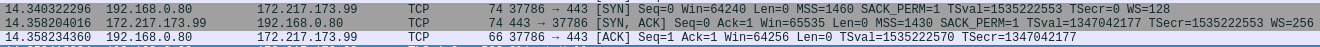
\includegraphics[width=\linewidth]{inicio.png}
    \caption{Estabelecimento de conexão.}
\end{figure}

\subsection{Tráfego da conexão}

Após ter a comunicação estabelecida pelo protocolo HTTP, a transmissão de dados pelas duas fontes pode ser realizada por diversos protocolos, aqui foi escolhido o HTTP, por ser o protocolo utilizado pelo Youtube e outras plataformas. O TLS em si possui uma camada de criptografia e um handshake separado além do que já foi realizado pelo TCP.

Após finalizados os procedimentos de segurança os dados podem ser trafegados no mesmo modelo do protocolo HTTP comum, com \emph{headers} e um \emph{body}, além de outros metadados. O TLS possui um \emph{keep-alive}, então múltiplas transmissões de dados podem ser realizadas a partir de um mesmo handshake. Na figura 2 podemos ver os pacotes que foram utilizados desde o início do handshake TLS até as transmissões de dados realizadas.

\begin{figure}[H]
    \centering
    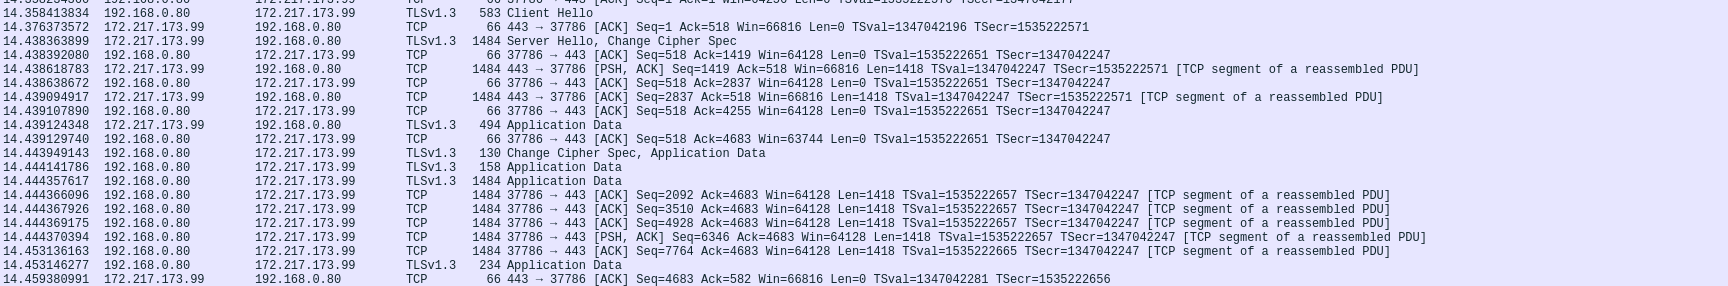
\includegraphics[width=\linewidth]{transmissao.png}
    \caption{Protocolo HTTP transmitindo dados.}
\end{figure}

\subsection{Encerrando conexão HTTP}

O final de uma conexão do protocolo HTTP necessita de uma série procedimentos e acordos, conforme descrito previamente. Na figura 3 podemos ver isso acontecendo diversas vezes em conexões diferentes. Perceba o envio de um FIN/ACK que depois é respondido com FIN/ACK para finalizar completamente a conexão.

\begin{figure}[H]
    \centering
    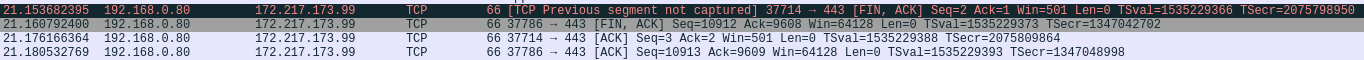
\includegraphics[width=\linewidth]{final.png}
    \caption{Finalizando conexão HTTP.}
\end{figure}

\section{Funcionamento do protocolo UDP e experimento}
\subsection{Detalhamento protocolo UDP}
A razão básica é que o UDP é um protocolo sem conexão ao contrário do TCP. O protocolo de datagramas do usuário (UDP) opera sobre o protocolo da Internet (IP) para transmitir datagramas em uma rede. O UDP não exige que a origem e o destino estabeleçam um handshake triplo antes que a transmissão ocorra. Além disso, não há necessidade de uma conexão de ponta a ponta.

O UDP é considerado um protocolo sem conexão porque não exige que um circuito virtual seja estabelecido antes que qualquer transferência de dados ocorra. O protocolo de comunicação apenas envia os pacotes, o que significa que ele tem muito menos sobrecarga de largura de banda e latência.

Com isso, os pacotes podem seguir caminhos diferentes entre o emissor e o receptor e, como resultado, alguns pacotes podem ser perdidos ou recebidos fora de ordem. Desse modo, existem muitos protocolos que usam UDP, entre eles: DNS, DHCP, BOOTP, TFTP, RIP, Protocolo em tempo real que não tolera atrasos, \emph{multicast} e etc.

\subsection{Desenvolvimento do experimento com protocolo UDP}
De acordo com Bamdeb Ghosh \cite{linuxhint}, O UDP fornece dois serviços não fornecidos pela camada IP, um deles é o número da porta e outro é um recurso de soma de verificação para identificar se os dados estão intactos.

O cabeçalho UDP contêm 8 bytes e possui:
 \begin{itemize}
   \item Porta de origem: O número da porta de origem do pacote. Exemplo: 4444.
   \item Porta de destino: O número da porta de destino do pacote. Exemplo: 51164.
   \item Comprimento: O comprimento dos dados UDP mais cabeçalho UDP.
   \item Checksum: Detecta o erro. 
 \end{itemize}

Para realizar a análise através do Wireshark, foi utilizado o serviço de streaming de vídeo Twitch, conforme a figura 4:

\begin{figure}[H]
    \centering
    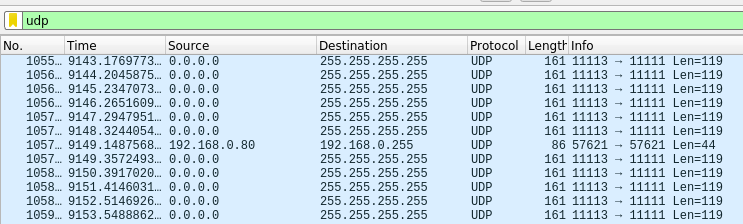
\includegraphics[width=\linewidth]{udp.png}
    \caption{Protocolo UDP trafegando dados.}
\end{figure}

Esmiuçando os segmentos, na figura 5 foi possível identificar os cabeçalhos e os dados do pacote:
\begin{figure}[H]
    \centering
    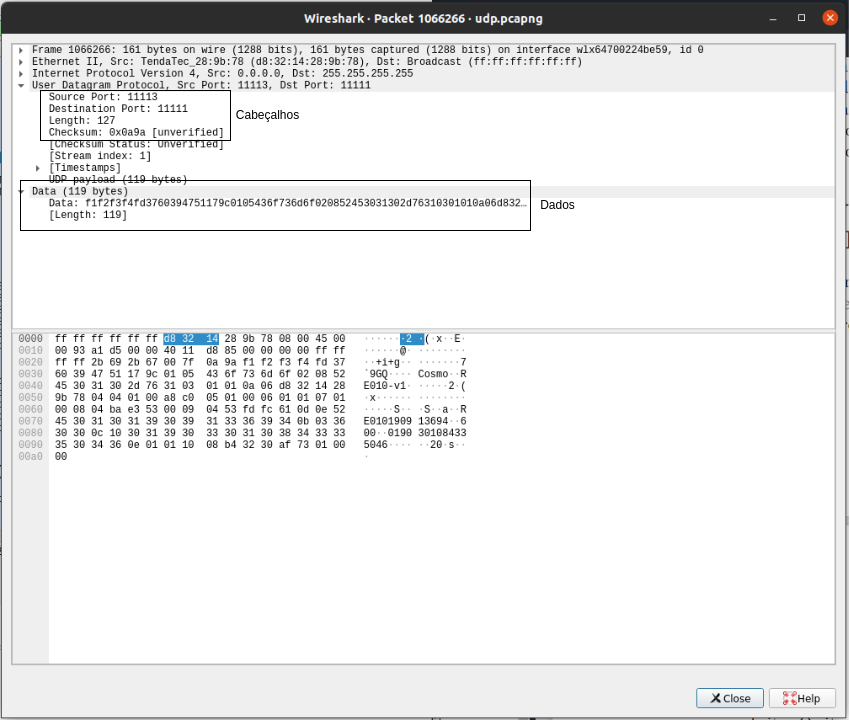
\includegraphics[width=\linewidth]{header_data.png}
    \caption{Protocolo UDP análise de cabeçalhos e dados.}
\end{figure}

\section{Conclusão}

Realizando esse trabalho foi possível perceber na prática o funcionamento de protocolos que fundamentam a rede mundial de computadores e a vida de todos nós. O uso da ferramenta Wireshark, bem como do protocolo HTTP, junto com o TCP permitiu a experiência prática e uma maior conhecimento da gerência de redes e desses protocolos utilizados. Em suma, o trabalho cumpriu seus requisitos pedagógicos e didáticos para a formação de um profissional da ciência da computação.

\nocite{*}
\medskip

\bibliographystyle{abbrv}
\bibliography{biblio}
\end{document}